\documentclass{article}

\usepackage{graphicx}
\usepackage{hyperref}
\graphicspath{ {./images/} }
\title{
  \huge
  \textbf{Buku Panduan Proxmox}
  \\
  \huge
  Instalasi Pada Server
}

\author{
  \textsc{Classroom Dev Team}
}

\begin{document}
  \pagenumbering{gobble}
  \maketitle

  \newpage
  \pagenumbering{roman}

  \newpage
  \pagenumbering{arabic}
  \section{Proses Instalasi}
  \subsection{Download ISO}
  ISO Proxmox dapat didownload melalui wesite resmi proxmox. \url{https://www.proxmox.com/en/downloads}
  dibawah ini merupakan website proxmox.
  \begin{figure}[h!]
    \centering
    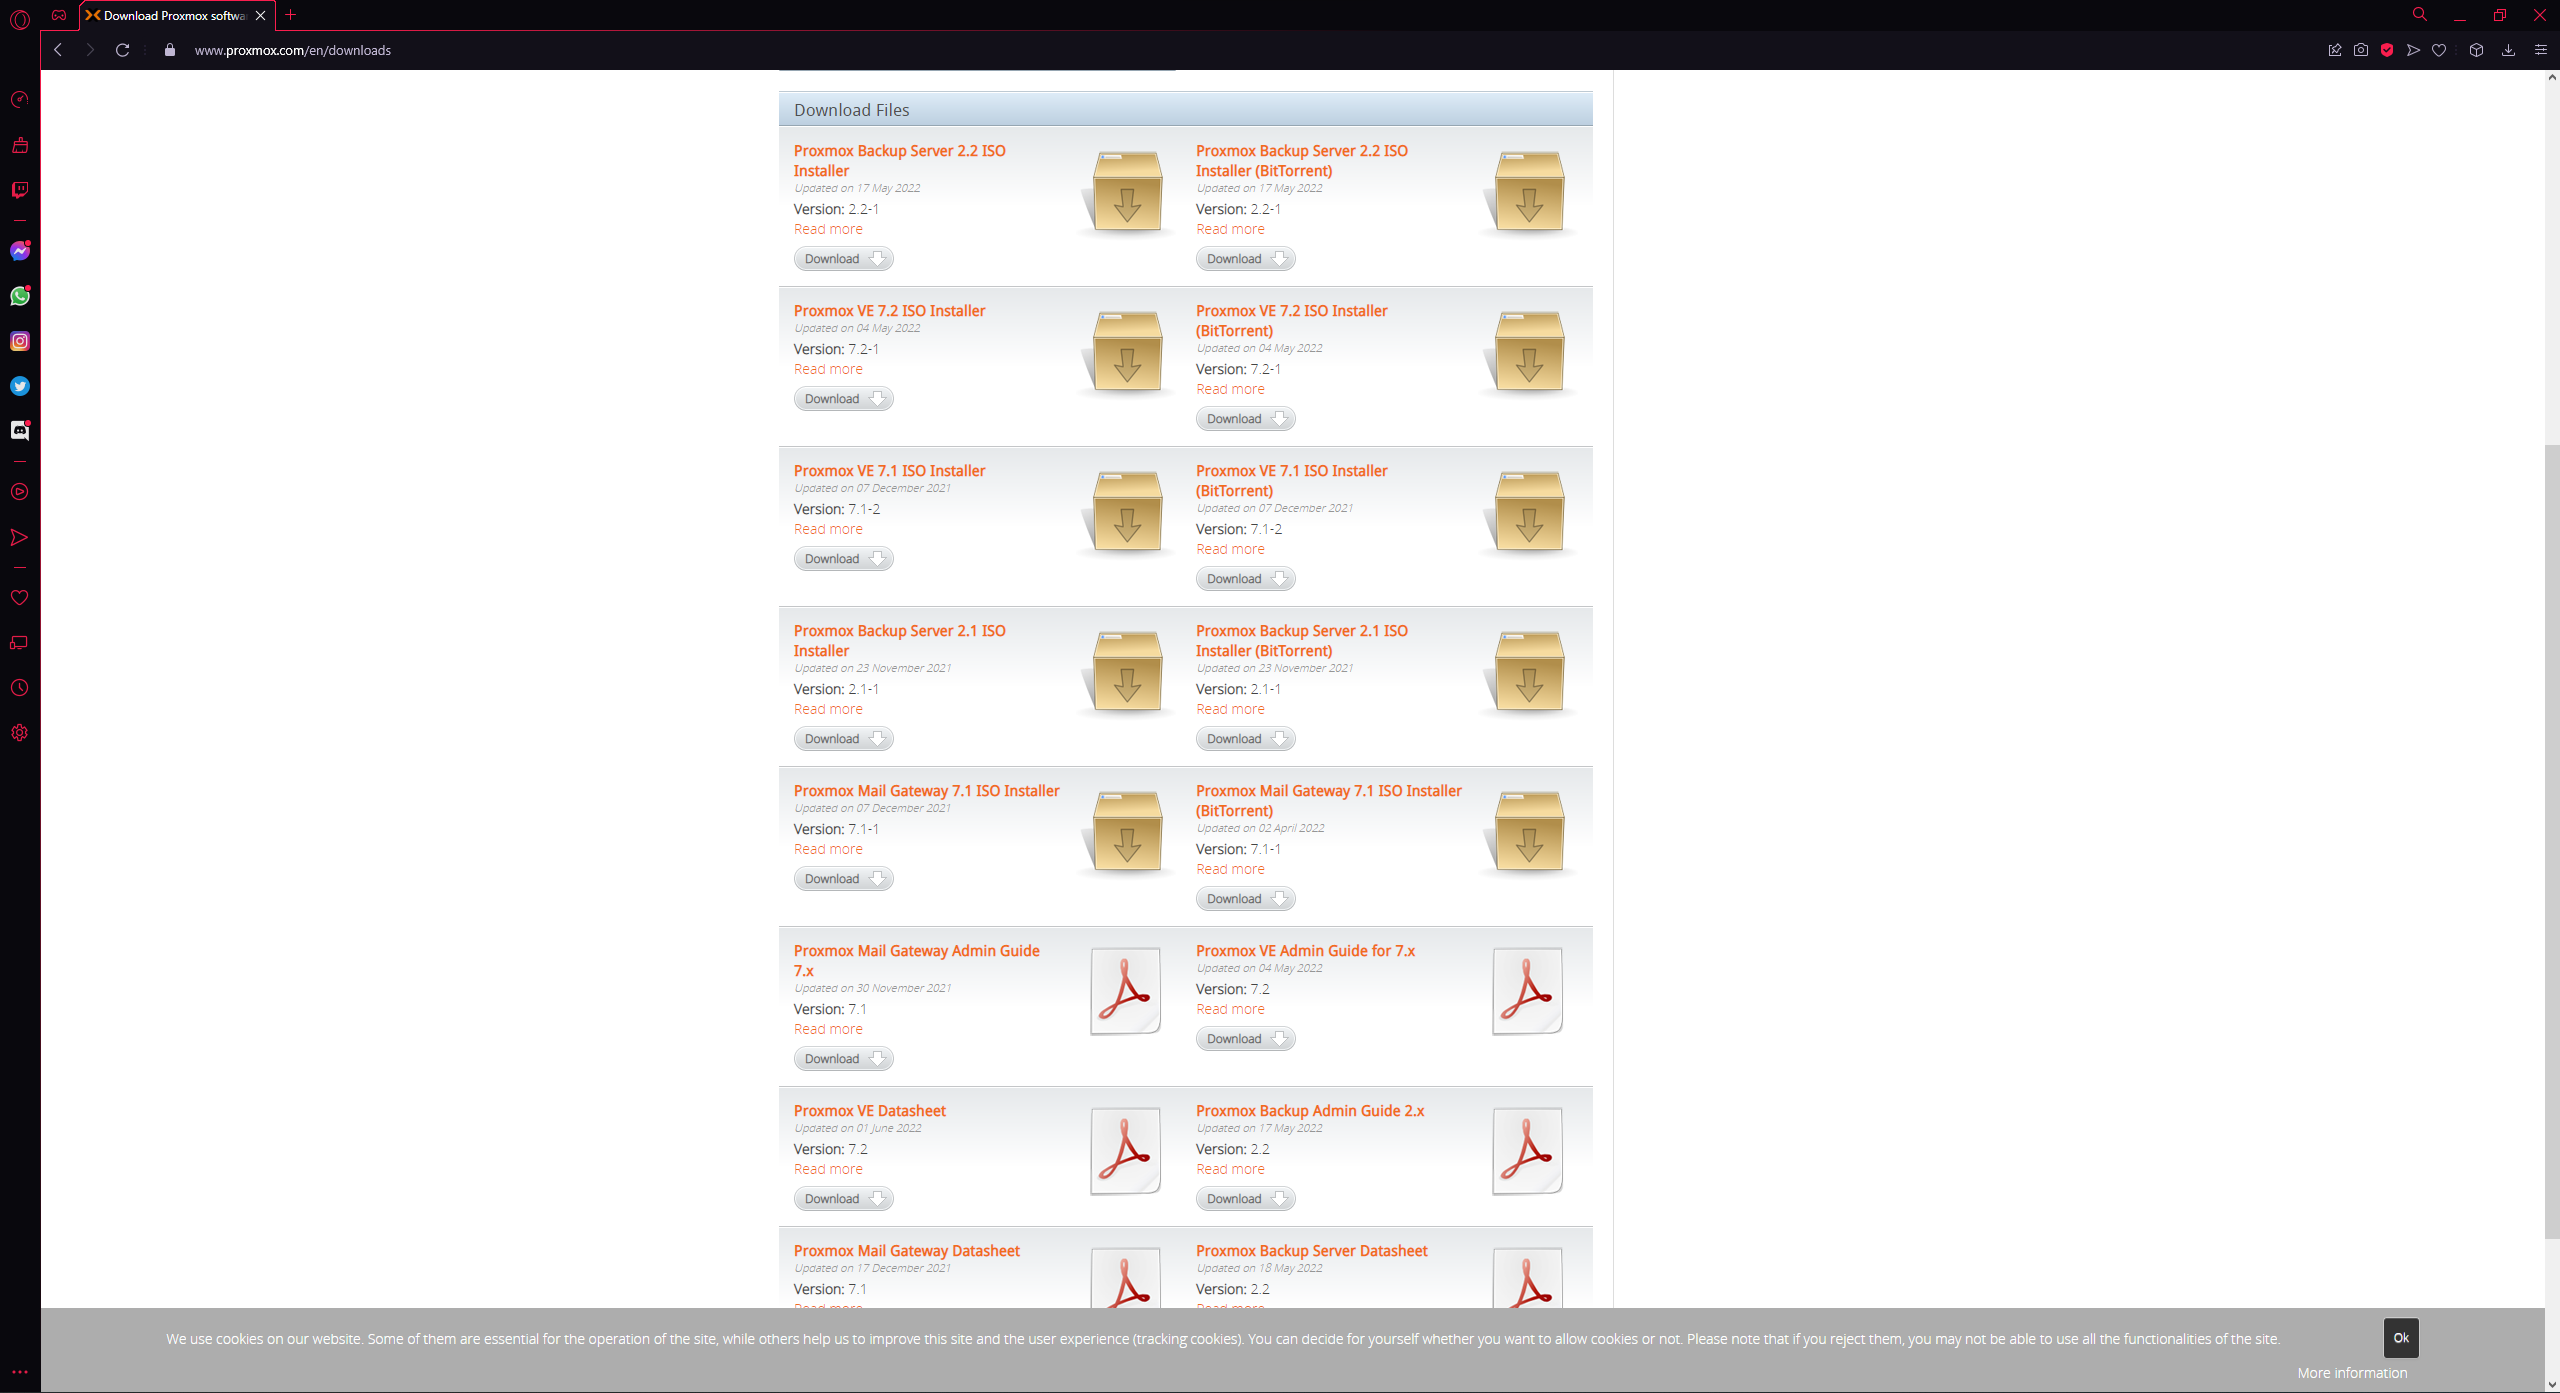
\includegraphics[width=1\linewidth]{proxmox web.png}
    \caption{web proxmox}
  \end{figure}
  \\ Setelah masuk ke website proxmox, tekan download pada salah satu list. Disarankan untuk mendownload Proxmox VE 7.1 ISO Installer
  \begin{figure}[h!]
    \centering
    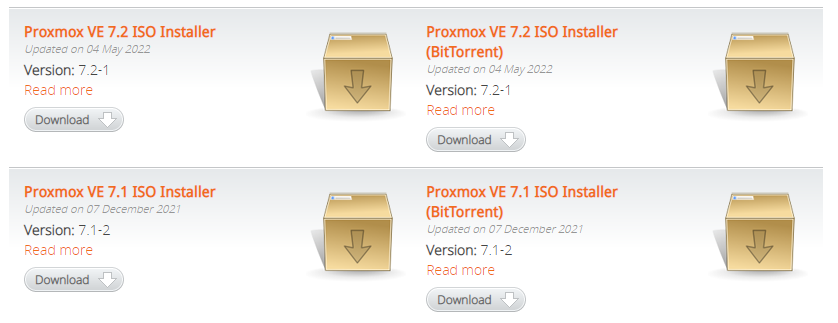
\includegraphics[width=1\linewidth]{proxmox download.png}
    \caption{download ISO}
  \end{figure}

  \newpage
  \subsection{Membuat Bootable}
  Pada proses pembuatan bootable ISO proxmox yang telah didownload akan dimasukkan ke USB flashdisk melalui proses flash menggunakan aplikasi balenaEtcher. 
  Aplikasi tersebut dapat didownload di \url{https://www.balena.io/etcher/}
  \begin{figure}[h!]
    \centering
    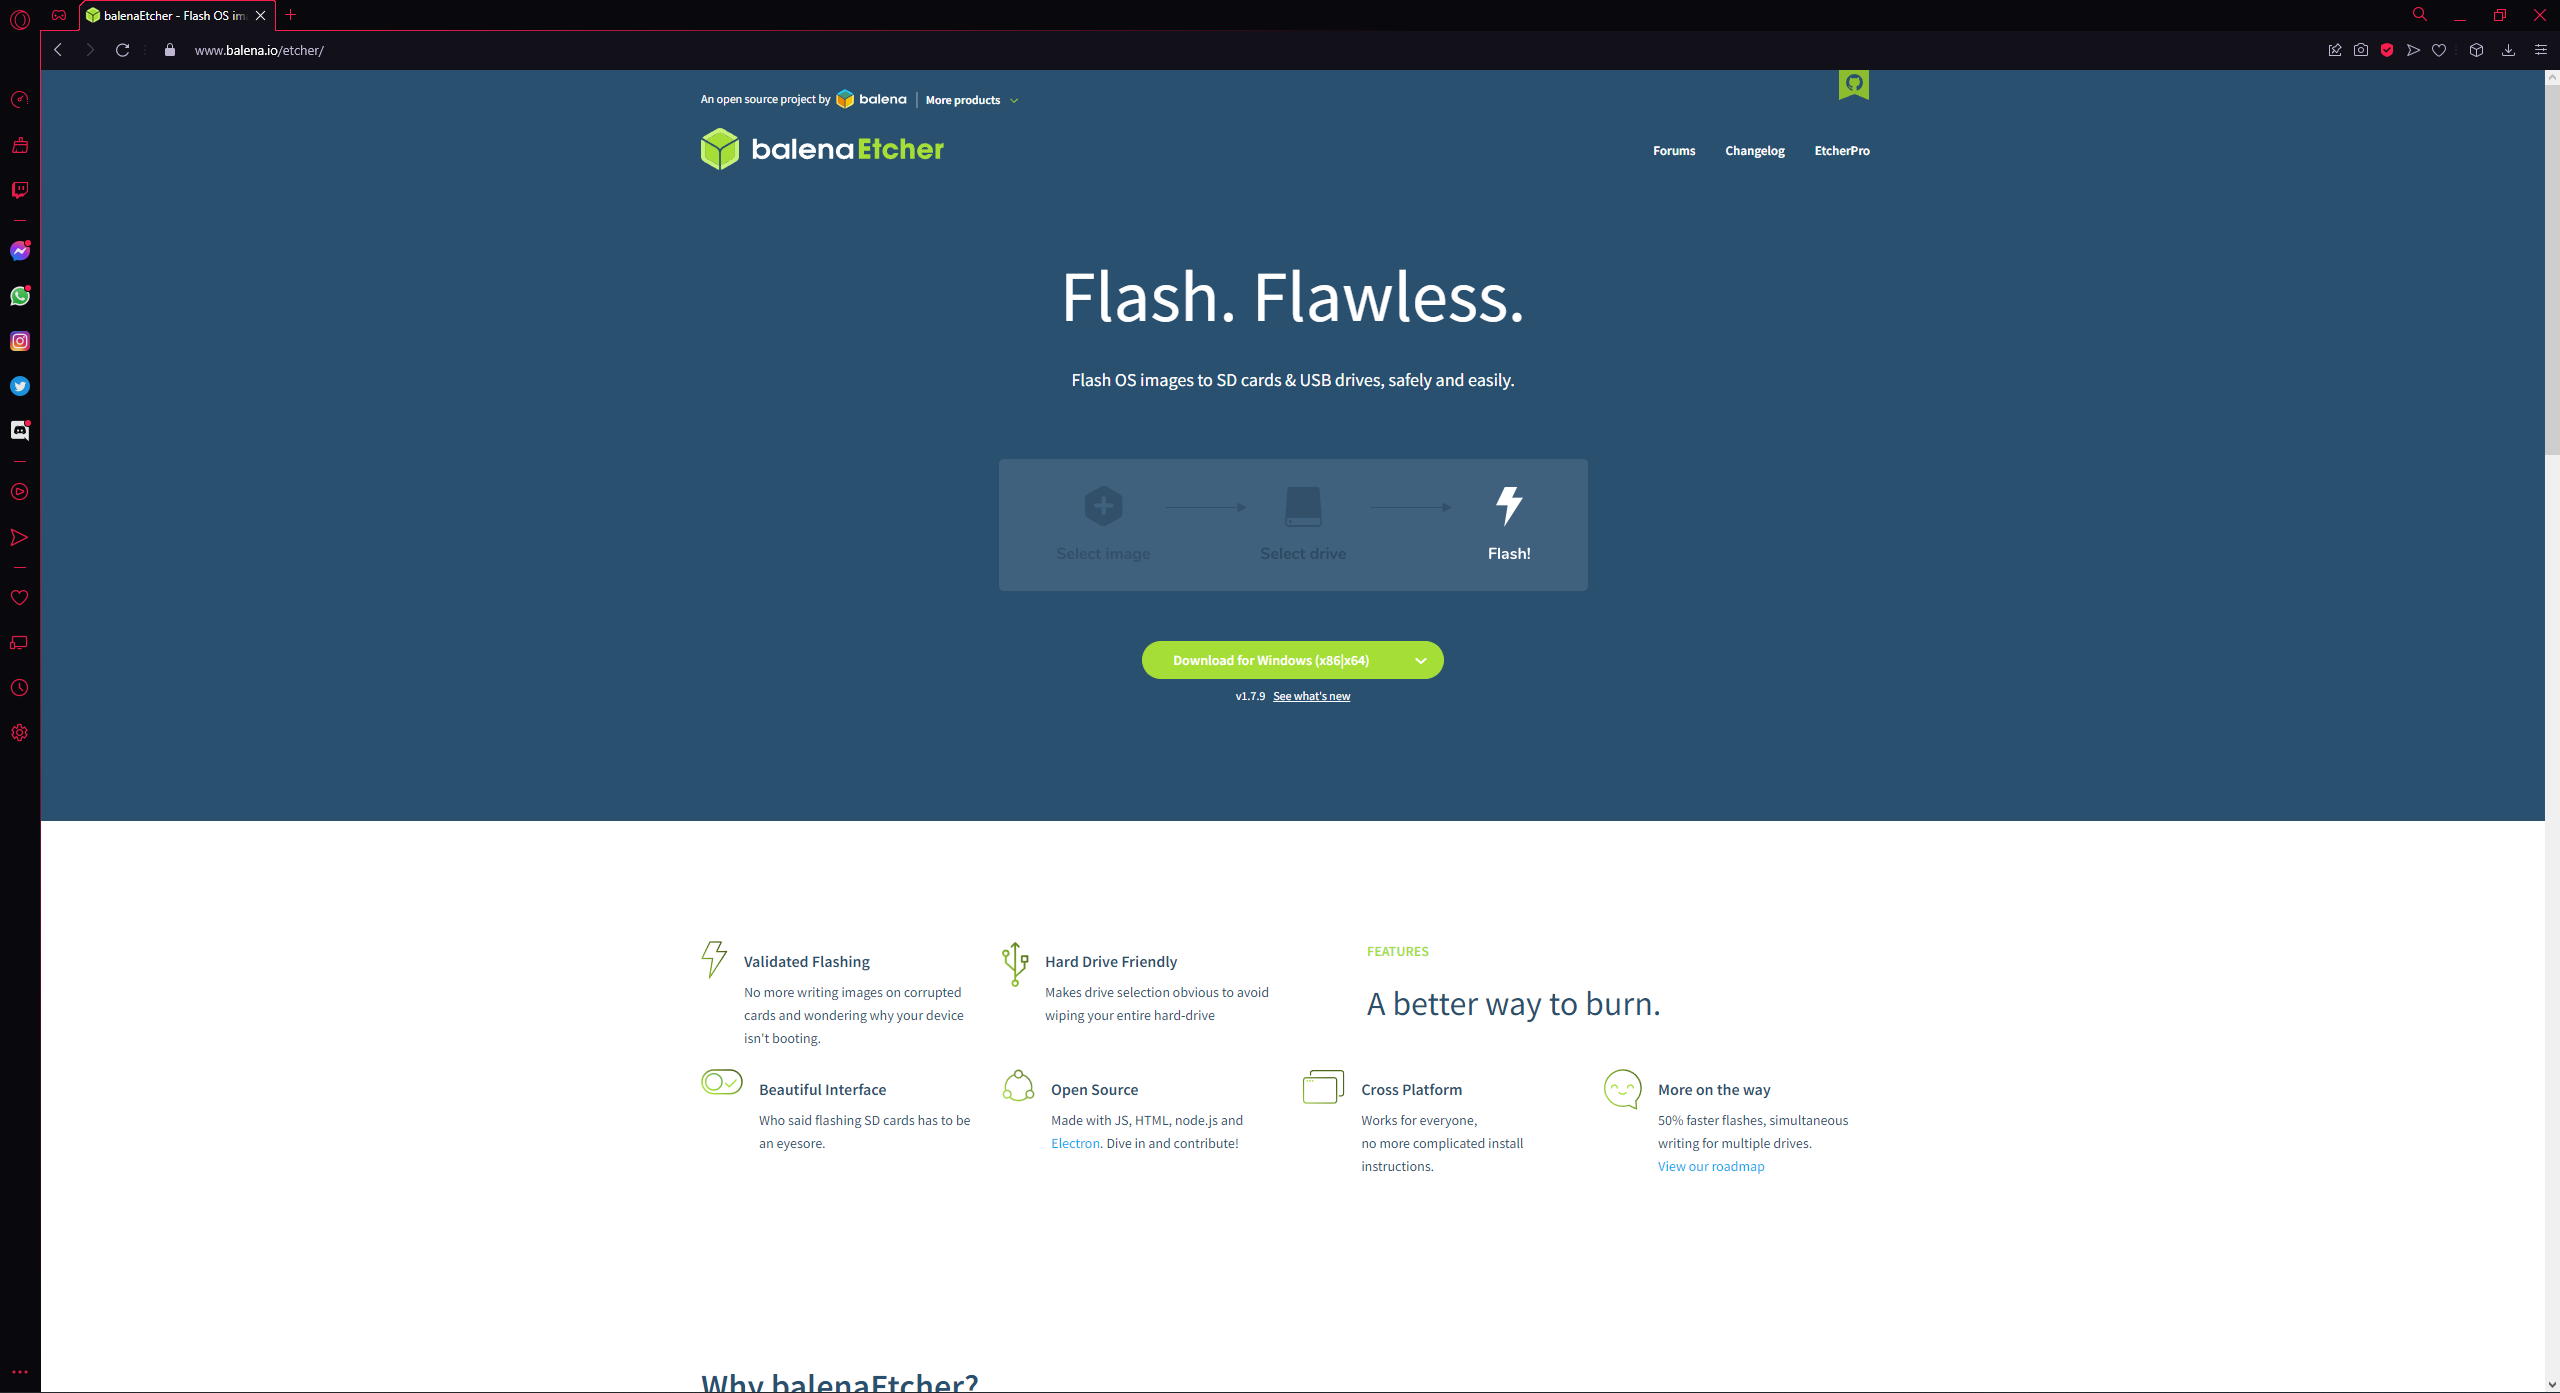
\includegraphics[width=0.9\linewidth]{balena web.png}
    \caption{web balena}
  \end{figure}
  \\ Setelah itu download aplikasi balenaEtcher sesuai sistem operasi yang digunakan. 
  Setelah proses download selesai maka lakukan instalasi aplikasi balenaEtcher,
  jika proses instalasi selesai maka akan muncul tampilan seperti berikut. Sambungkan USB flashdisk ke PC, 
  lalu pada aplikasi balenaEtcher pilih Flash from file,
  seteh itu pada Select target pilih USB flashdisk, lalu Flash!
  \begin{figure}[h!]
    \centering
    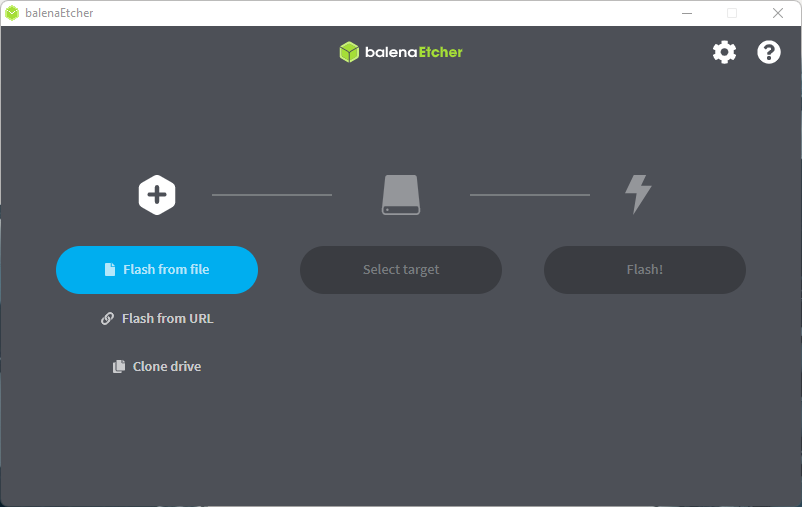
\includegraphics[width=0.75\linewidth]{balena.png}
    \caption{aplikasi balena}
  \end{figure}
  \\ Jika terdapat error pada proses bootable maka matikan terlebih dahulu windows firewall.
  \begin{figure}[h!]
    \centering
    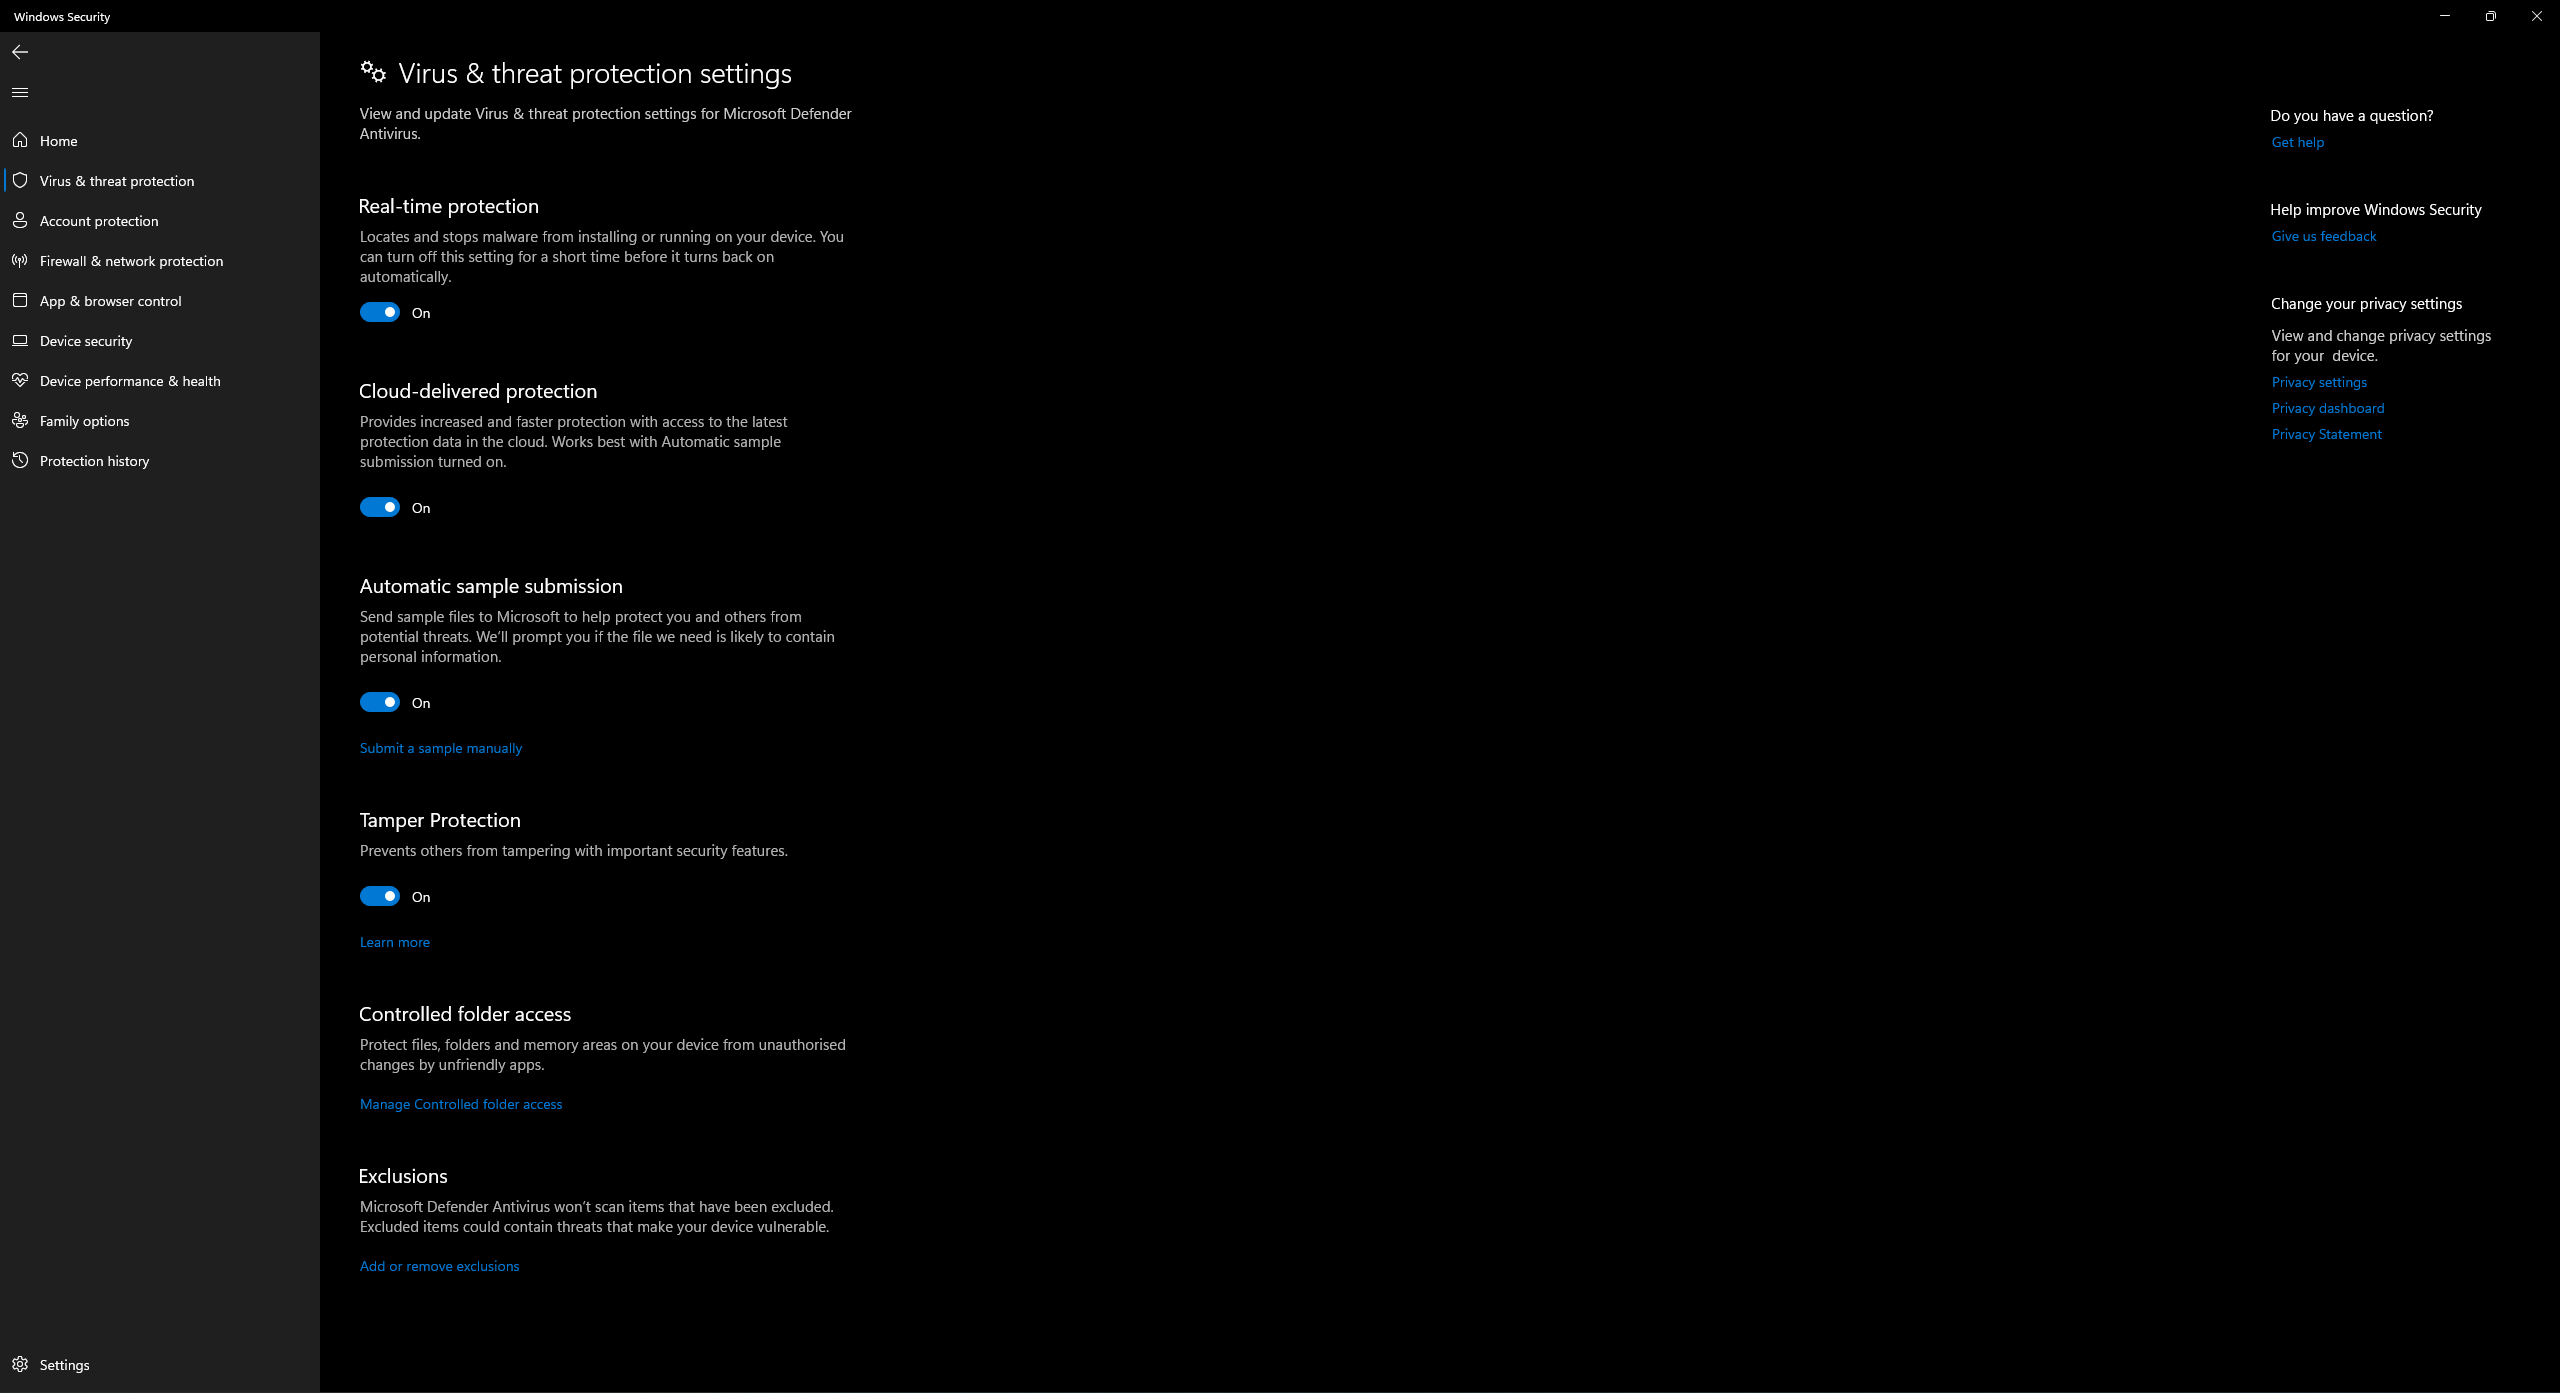
\includegraphics[width=0.7\linewidth]{firewall.png}
    \caption{firewall}
  \end{figure}
  \\ Setelah proses bootable, pasangkan USB flashdisk pada PC yang akan diinstall proxmox. Ubahlah proses Boot pada PC dengan memasuki BIOS atau UEFI,
  lalu masuk ke menu Boot atau System Configuration dan pilih Boot Order/Hard drive BBS Priorities. Pastikan Boot USB berada dipaling atas
  \newpage

  \subsection{Instalasi Proxmox}
  Setelah memasuki Boot pada USB flashdisk maka akan muncul tampilan seperti berikut. Berikut merupakan langkah - langkah instalasi :
  \begin{enumerate}
    \item Pilih Install Proxmox VE
    \begin{figure}[h!]
      \centering
      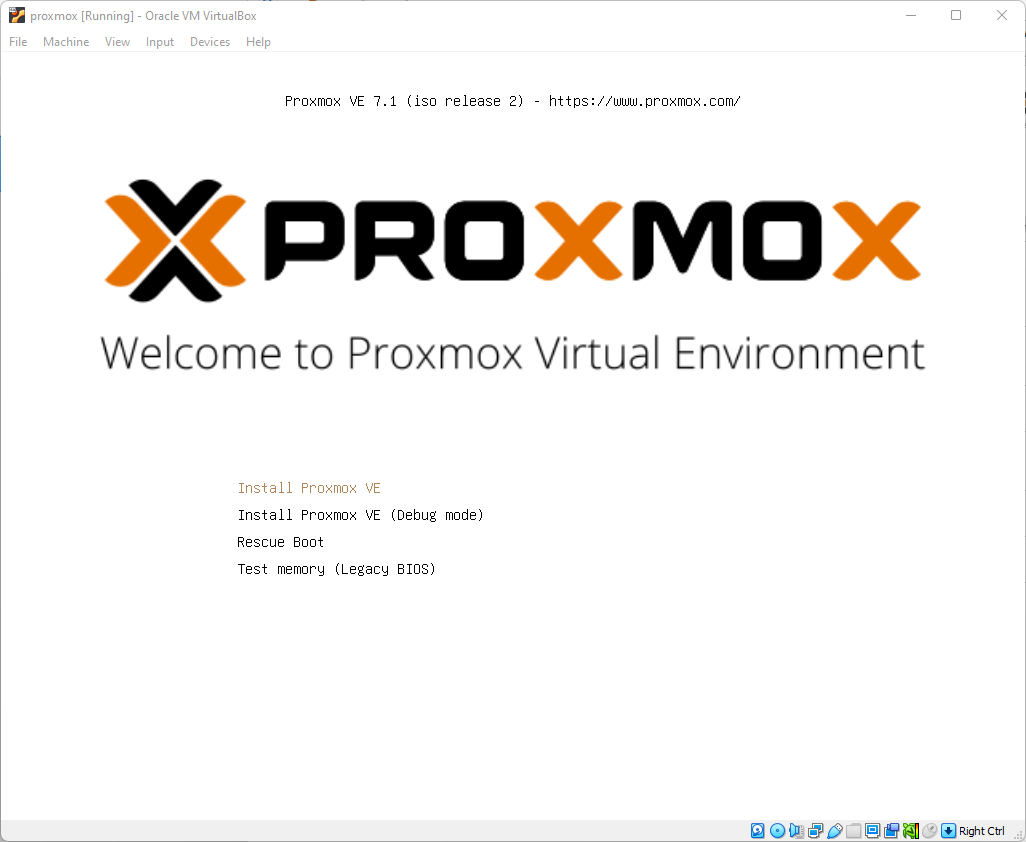
\includegraphics[width=0.7\linewidth]{proxmox 1.png}
      \caption{Proxmox 1}
    \end{figure}
    \newpage
    \item Tekan OK
    \begin{figure}[h!]
      \centering
      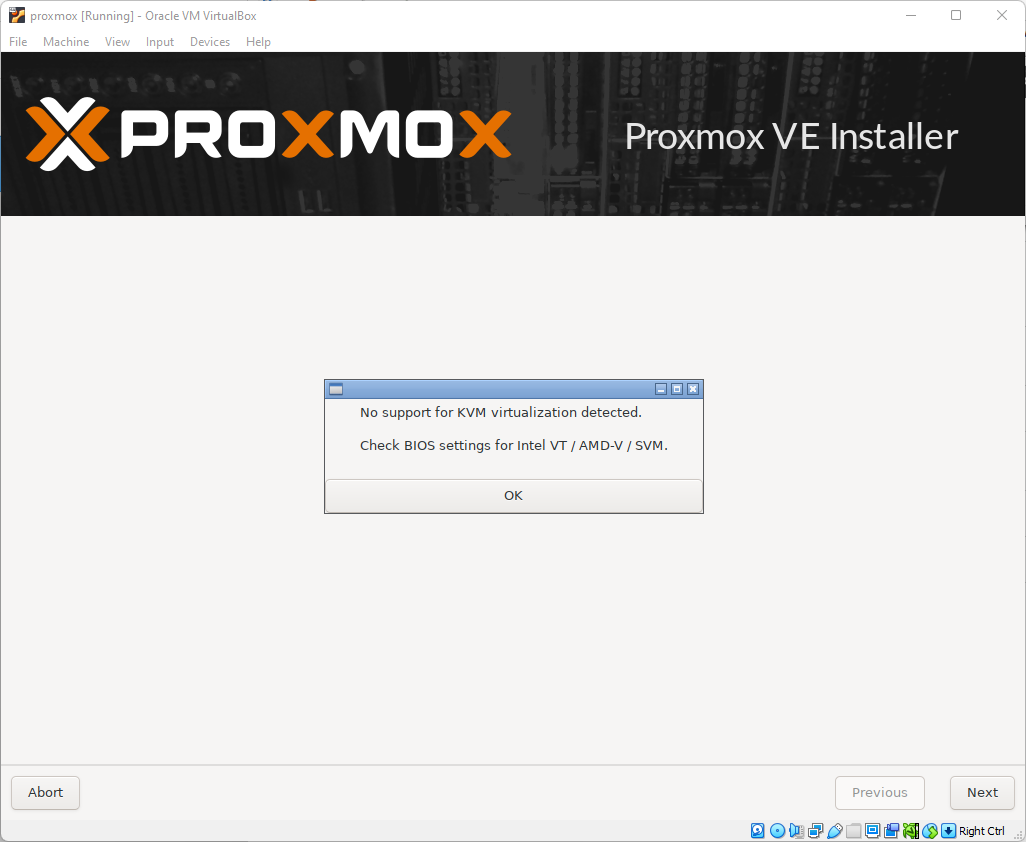
\includegraphics[width=0.7\linewidth]{proxmox 2.png}
      \caption{Proxmox 2}
    \end{figure}
    \item Tekan I agree
    \begin{figure}[h!]
      \centering
      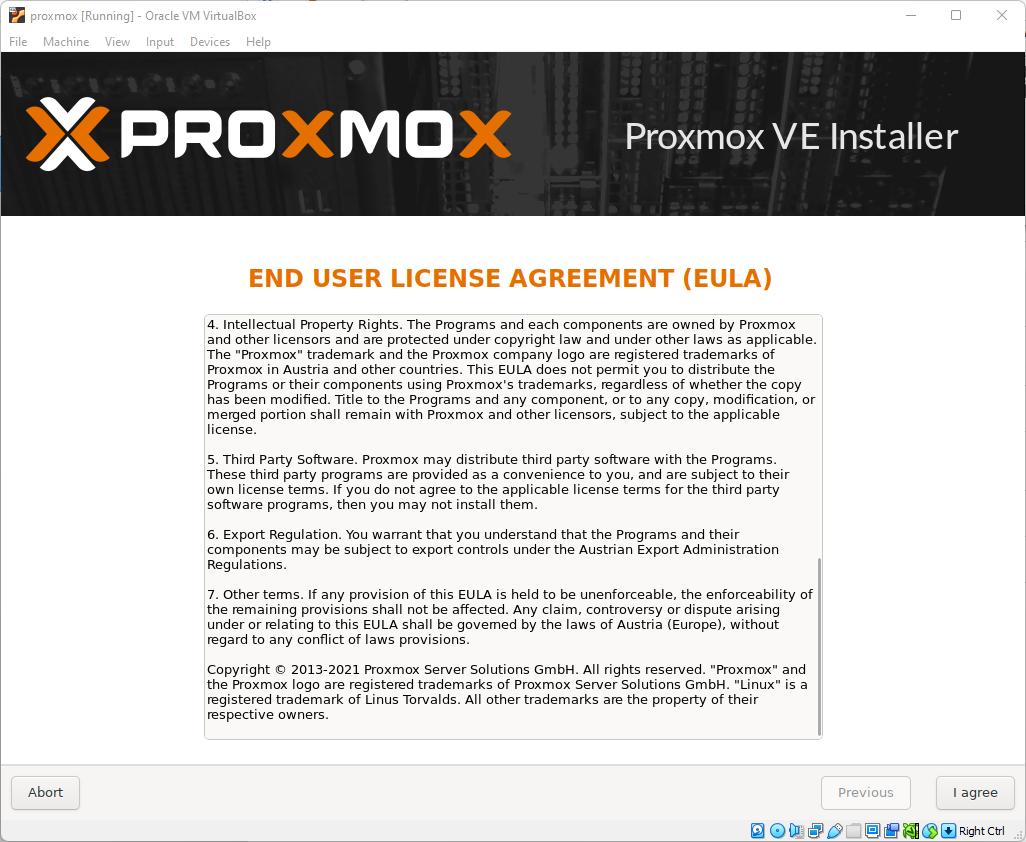
\includegraphics[width=0.7\linewidth]{proxmox 3.png}
      \caption{Proxmox 3}
    \end{figure}
    \newpage
    \item Pilih Target harddisk lalu tekan Next
    \begin{figure}[h!]
      \centering
      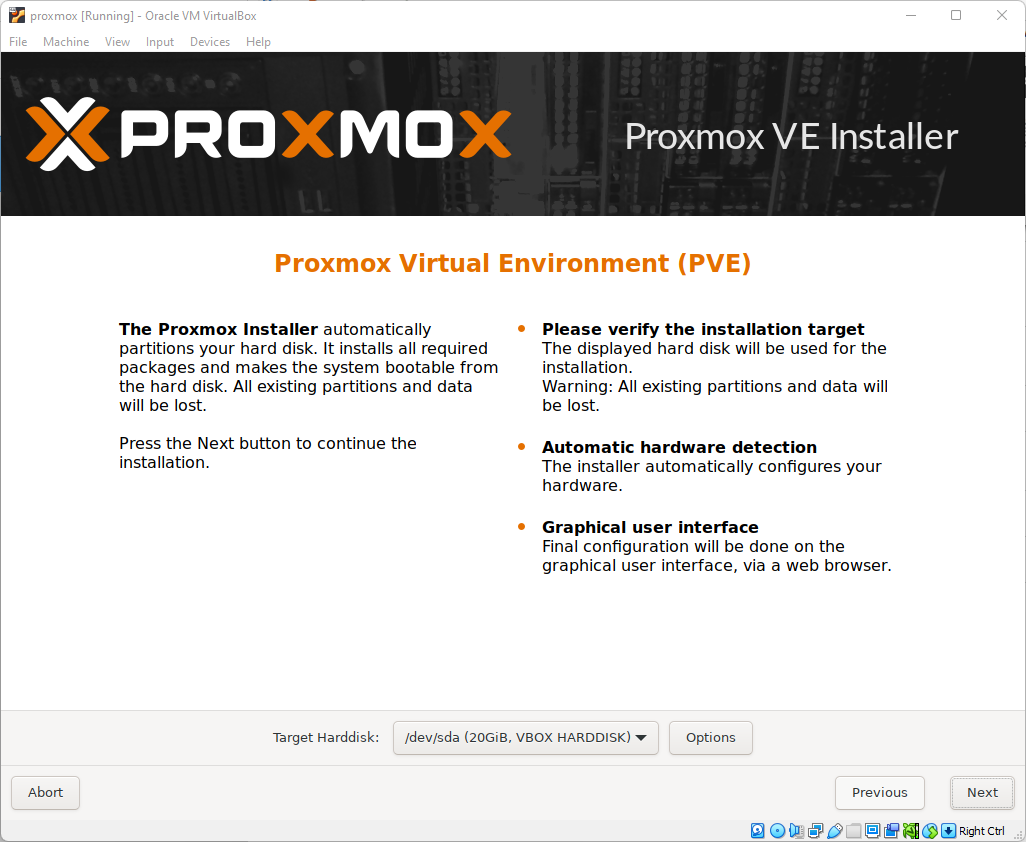
\includegraphics[width=0.7\linewidth]{proxmox 4.png}
      \caption{Proxmox 4}
    \end{figure}
    \item Pilih negara, zona waktu dan keyboard layout. Untuk keyboard layout biarkan saja menjadi U. S. English
    \begin{figure}[h!]
      \centering
      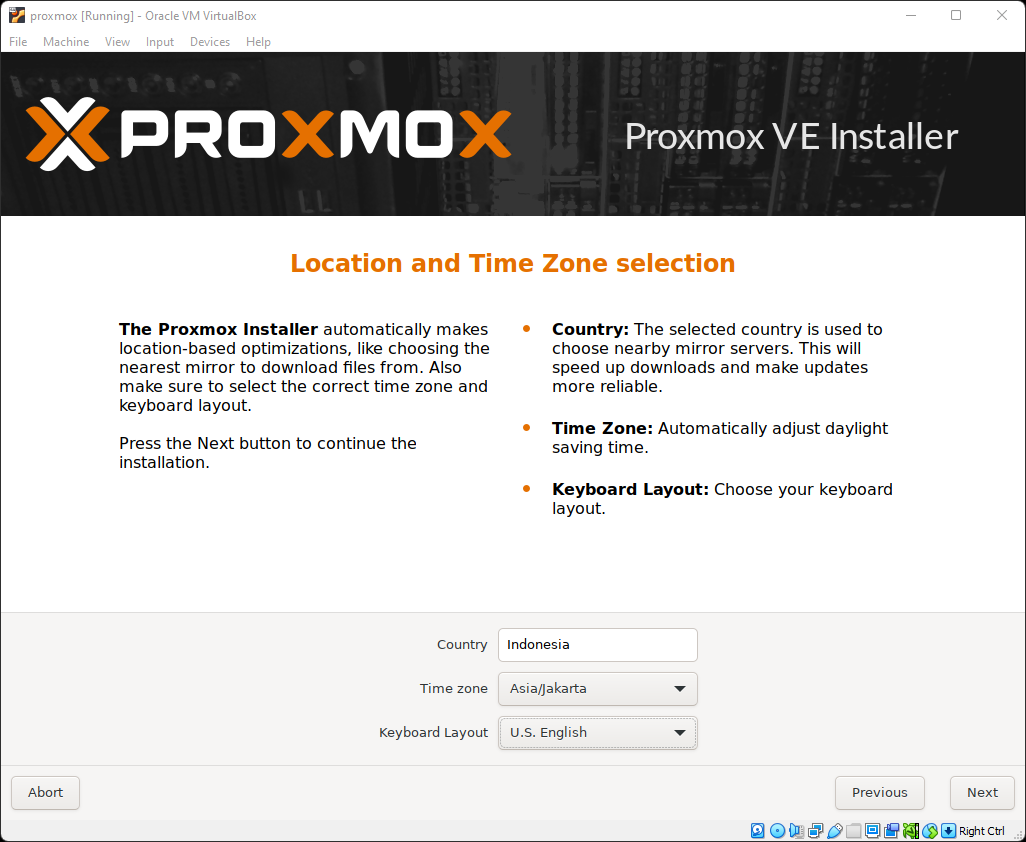
\includegraphics[width=0.7\linewidth]{proxmox 5.png}
      \caption{Proxmox 5}
    \end{figure}
    \newpage
    \item Masukkan password dan email
    \begin{figure}[h!]
      \centering
      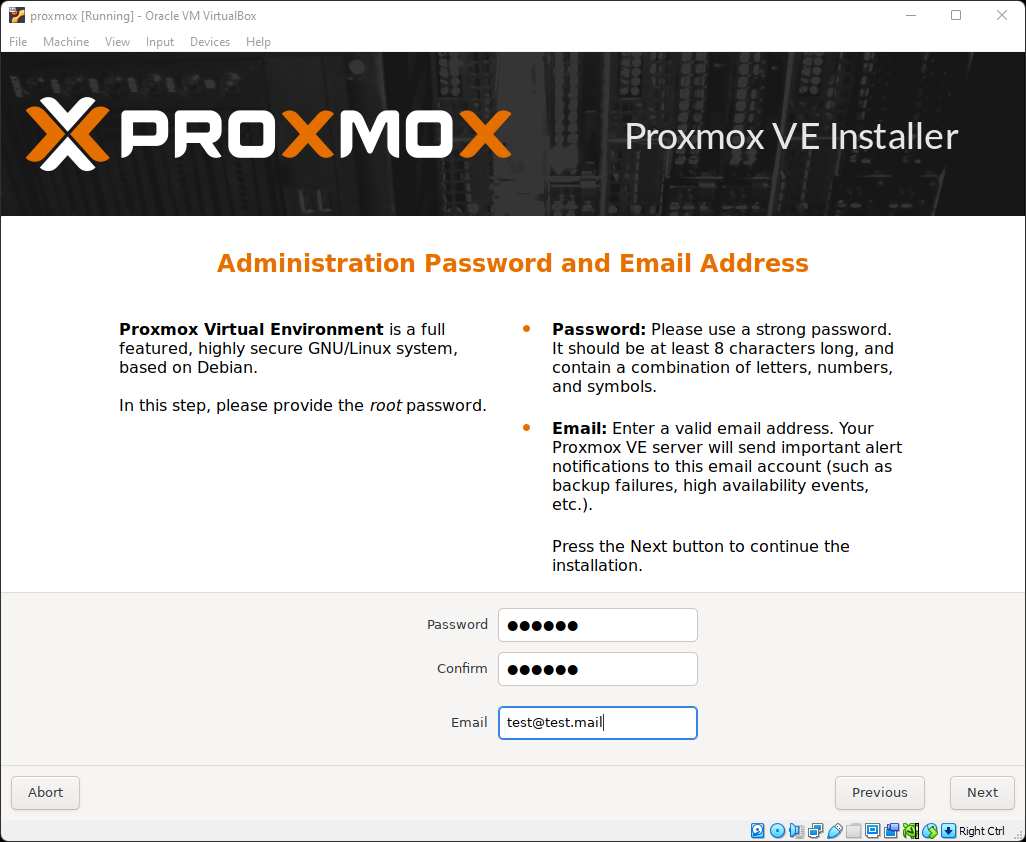
\includegraphics[width=0.7\linewidth]{proxmox 6.png}
      \caption{Proxmox 6}
    \end{figure}
  \end{enumerate}
\end{document}